%\section{The data ellipse and ellipsoids}\label{sec:data-ellipse}

The \emph{data ellipse} \citep{Monette:90} (or \emph{concentration ellipse}, \citealp[Ch. 7]{Dempster:69})
provides a remarkably
simple and effective display for viewing and understanding
bivariate \emph{marginal} relationships in multivariate data.
The data ellipse is typically used to add a visual summary to a scatterplot,
indicating the means, standard deviations, correlation,
and slope of the regression line for
two variables. Under classical (Gaussian) assumptions, the data ellipse
provides a statistically sufficient visual summary, as we describe below.


\begin{figure}[htb]
  \centering
  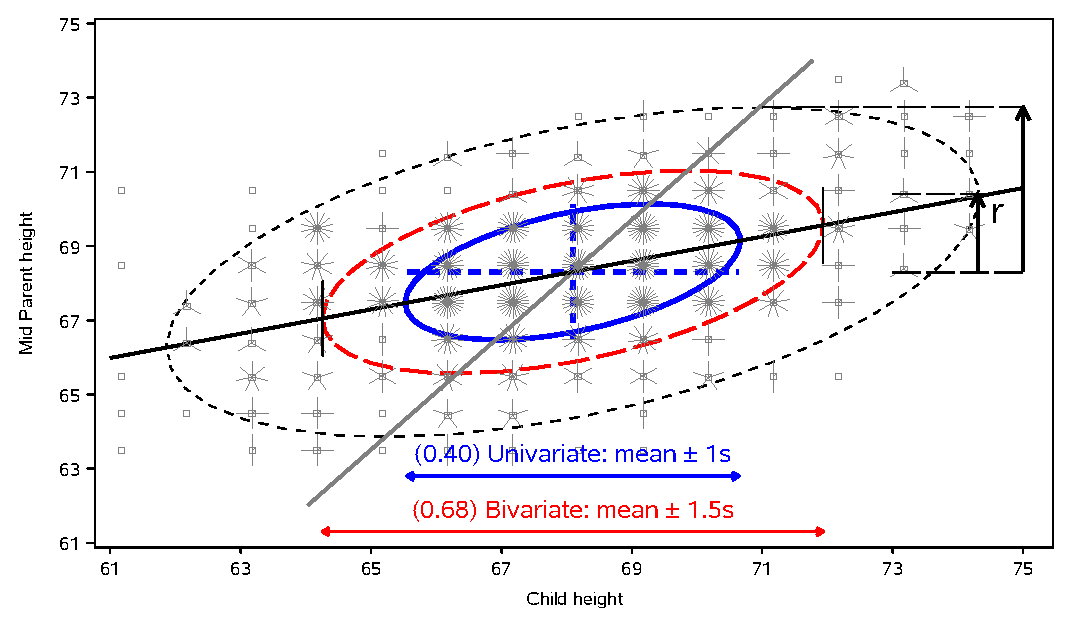
\includegraphics[width=.9\textwidth,clip]{fig/galton-reg3}
  \caption{Sunflower plot of Galton's data on heights of parents and their children (in.), with
  40\%, 68\% and 95\% data ellipses and the regression lines of $y$ on $x$ (black) and
  $x$ on $y$ (grey). The ratio of the vertical to the regression line (labeled `r') to the vertical
  to the top of the ellipse gives a visual estimate of the correlation ($r$=0.46, here).
  Shadows (projections) on the coordinate axes give standard intervals, with $k=1, 1.5, 2.45$,
  bivariate coverate 40\%, 68\% and 95\%, and univariate coverage 68\%, 87\% and 98.6\% respectively.
  $\bar{x} \pm k s_x$ and $\bar{y} \pm k s_y$, 
%with various coverage properties.
  Plotting children's height on the abscissa follows Galton.
  }%
  \label{fig:galton-reg3}
\end{figure}

It is historically appropriate to illustrate the data ellipse and
describe its properties using Galton's (\citeyear[Table
I]{Galton:1886})
data, from which he drew \figref{fig:galton-corr} as a conceptual
diagram,%
\footnote{These data are reproduced in \citet[Table 8.2, p.
286]{Stigler:1986}}
shown in \figref{fig:galton-reg3}, where the frequency at
each point is represented by a sunflower symbol. We also overlay the 40\%,
68\% and 95\% data ellipses, as described below.

In \figref{fig:galton-reg3}, the ellipses have the mean vector
$(\bar{x}, \bar{y})$ as their center;  the lengths of arms of the
central cross show the standard deviations of the variables, which
correspond to the shadows of the 40\% ellipse.  In
addition, the correlation coefficient can be visually represented as
the fraction of a vertical tangent line from $\bar{y}$ to the top of
the ellipse that is below the regression line $\widehat{y} | x$, shown
by the arrow labeled `r.' Finally, as Galton noted, the regression line
for $\widehat{y} \given x$ (or $\widehat{x} \given y$)
can be visually estimated as the locus of the points of vertical
(or horizontal) tangents with the family of concentric ellipses.
See \citet[Figs.~5.1--5.2]{Monette:90} and
\citet[p.~183]{Friendly:91} for illustrations and further discussion
of the properties of the data ellipse.

More formally \citep{Dempster:69,Monette:90}, for a $p$-dimensional
sample, $\mat{Y}_{n \times p}$,
we recognize the quadratic form in \eqref{eq:ellipsoid3}
as corresponding to the squared Mahalanobis distance,
$D^2_M (\vec{y}) = \dev{\vec{y}}\trans \, \inv{S} \, \dev{\vec{y}}$,
of the point
$\vec{y} = (y_1, y_2, \dots , y_p)\trans$
from the centroid of the sample,
$\bar{\vec{y}} = (\bar{y}_1, \bar{y}_2, \dots , \bar{y}_p)\trans$.
Thus, we use a more explicit notation to
define the \emph{data ellipsoid} $\mathcal{E}_c$ of size (``radius'') $c$
as the set of all points $\vec{y}$ with $D^2_M (\vec{y})$ less than or
equal to $c^2$,
\begin{equation}\label{eq:dsq}
\mathcal{E}_c ( \bar{\vec{y}},  \mat{S} )
:= \{ \vec{y} :
\dev{\vec{y}}\trans \, \inv{S} \, \dev{\vec{y}} \le c^2 \} \comma
\end{equation}
where
$\mat{S} = ({n-1})^{-1} \sum_{i=1}^n (\vec{y}_i - \bar{\vec{y}}) (\vec{y}_i - \bar{\vec{y}}\trans)$
is the sample covariance matrix.  In the computational notation of \eqref{eq:ellipsoidW}, the boundary of the
data ellipsoid of radius $c$ is thus
\begin{equation}\label{eq:ellipsoidS}
\mathcal{E}_c(\bar{\vec{y}}, \mat{S}) = \bar{\vec{y}} \oplus c \mat{S}^{1/2} \period
\end{equation}

Many properties of the data ellipsoid hold regardless of the joint distribution of the
variables; but if the variables are multivariate normal, then the data ellipsoid approximates
a contour of constant density in their joint distribution.  In this case $D^2_M (x,y)$
has a large-sample $\chi^2_p$ distribution, or, in finite samples, approximately
$[p (n-1) / (n-p)] F_{p, n-p}$).

Hence, in the bivariate case, taking $c^2 = \chi^2_2(0.95)= 5.99 \approx 6$ encloses approximately
95\% of the data points under normal theory.  Other radii also have useful interpretations:
\begin{itemize*}
\item In \figref{fig:galton-reg3}, we demonstrate that $c^2 = \chi^2_2(0.40) \approx 1$ gives
a data ellipse of 40\% coverage with the property that its projection on either axis
corresponds to a standard interval, $\bar{x} \pm 1 s_x$ and $\bar{y} \pm 1 s_y$.  The same property of univariate
coverage pertains to
any linear combination of $x$ and $y$.
\item By analogy with a univariate sample, a 68\% coverage data ellipse with
$c^2 = \chi^2_2(0.68) = 2.28$ gives a bivariate analog of the standard $\bar{x} \pm 1 s_x$ and $\bar{y} \pm 1 s_y$ intervals.
The univariate shadows, or those of any linear combination, then correspond to standard Scheff\'e
intervals taking ``fishing'' (simultaneous interfence) in a $p=2$-dimensional space into account.
\end{itemize*}


\begin{figure}[htb]
% two figs side-by-side
  \begin{minipage}[c]{.485\textwidth}
   \includegraphics[width=1\linewidth,clip]{fig/scatirisd1}
   \end{minipage}%
  \hfill
  \begin{minipage}[c]{.485\textwidth}
   \includegraphics[width=1\linewidth,clip]{fig/scatirisd3}
  \end{minipage}
  \caption{Scatterplot matrices of Anderson's iris data: (a) showing data, separate 68\% data
  ellipses, and regression lines for each species; (b) showing only ellipses and regression lines.
  Key-- \emph{Iris setosa}: blue, $\triangle$; \emph{Iris versicolor}: red, $+$;
  \emph{Iris virginca}: green, $\Box$.}%
  \label{fig:scatirisd1}
\end{figure}

As useful as the data ellipse might be for a single, unstructured
sample, its value as a visual summary increases
with the complexity of the data.
For example, \figref{fig:scatirisd1} shows  scatterplot matrices
of all pairwise plots of the variables from Edgar Anderson's \citeyear{Anderson:35}
classic
data on three species of iris flowers found in the Gasp\'{e} Peninsula,
later used by \citet{Fisher:36} in his development of discriminant analysis.
The data ellipses show clearly that the means, variances, correlations,
and regression slopes differ systematically across the three iris species
in all pairwise plots.
We emphasize that the ellipses serve as sufficient visual summaries of the important
statistical properties (first and second moments)% 
\footnote{
We recognize that a normal-theory summary (first and second moments),
shown visually or numerically, can be distorted
by multivariate outliers, particularly in smaller samples.
In what follows,
robust covariance estimates can, in principle, be substituted
for the classical, normal-theory estimates in all cases.
% Such effects can be countered by using
% robust covariance
% estimates such as multivariate trimming \citep{GnanadesikanKettenring:72}
% or the high-breakdown bound Minimum Volume Ellipsoid (MVE) and
% Minimum Covariance Determinant (MCD) methods
% developed by Rousseeuw and others
% \citep{RousseeuwLeroy:87,RousseeuwVanDriessen:99}.
% In what follows, it should be noted that
% robust covariance estimates could, in principle, be substituted
% for the classical, normal-theory estimates in all cases.
To save space, we don't explore these possibilities further here.
}
by removing the data points
from the plots in the version at the right.

%\subsection{Robust data ellipsoids}

